\documentclass[a4paper]{jacow}

\usepackage[utf8]{inputenc}
\usepackage[english]{babel}			 
\usepackage[final]{pdfpages}
\usepackage{lmodern}
\usepackage{multirow}
\usepackage{ragged2e}
\usepackage{amsmath, amssymb}
\usepackage{tikz}
\usepackage{xcolor}
\usepackage{siunitx}
%\usepackage{parskip}


% color definitions, mainly derived from the maincolor and black
\definecolor{maincolor}{cmyk}{10,75,0.0,0.0}
\colorlet{sensorcolor}{maincolor}
\colorlet{weightcolor}{maincolor!50}
\colorlet{outerblockcolor}{maincolor!30}

\colorlet{irrelevantcolor}{black!10}
\colorlet{midblockfillcolor}{black!10}
\colorlet{midblockdashedbordercolor}{black!50}

% used tikz librarys
\usetikzlibrary{
  arrows,
  shapes.misc,
  shapes,
}

% style definitions for the block diagram
\tikzstyle{basicblock}=[thick, draw, minimum height=2em]
\tikzstyle{vsinnerblock}=[basicblock, rectangle]
\tikzstyle{cinnerblock}=[basicblock, rounded rectangle]
\tikzstyle{outerblock}=[basicblock, fill=outerblockcolor, text width=5em,text centered, minimum height=20em, rounded corners]
\tikzstyle{midblocks}=[outerblock, draw=midblockdashedbordercolor, fill=midblockfillcolor, minimum height=8em, minimum width=20em, text width=10em]

\begin{document}

\title{Investigation of Nature Inspired Algorithms in a practical context by exploiting the characteristics of Braitenberg Vehicle Concepts}

\author{A. Dorn\thanks{andrea.dorn@uni-rostock.de}, University of Rostock, Germany \\
		H. Pommerenke\thanks{hermann.pommerenke@uni-rostock.de}, University of Rostock, Germany \\
		T. Steinmetz\thanks{tino.steinmetz@uni-rostock.de}, University of Rostock, Germany}
	
\maketitle

%\begin{abstract}
%   Insert shiny abstract!
%\end{abstract}

\section{The Braitenberg Vehicle}

The term Braitenberg Vehicle (BV) describes a vehicle which is capable of autonomous movement via two independent motors by considering primitive sensor inputs only.

These sensors typically are proximity or light sensors, but may also include gas, acoustic, and similar sensors for specific applications. Movement is achieved by calculating the motor speed $v$ as a linear combination of the sensor inputs $I$. Therefore, the values collected by the sensors are multiplied with weights $w$ and superimposed for each motor individually. Equation~(\ref{eq:motorequation}) shows this principle, where the index $n\in\{\mathrm{L},\mathrm{R}\}$ describes the corresponding motor and $i=0,\ldots,N-1$ denotes the individual sensor. To ensure a net forward movement, an additional bias $w_{n,\text{bias}}$ is added.
\begin{equation}
	v_{n} = \sum\limits_{i=0}^{N-1} w_{n,i}\cdot I_{i} + w_{n,\text{bias}}
	\label{eq:motorequation}
\end{equation}

The BV's behaviour can now be varied by adjusting the weights $w$. Considering a vehicle with $N$ sensors, this requires $2N+2$ weight values to be found, i.e. an optimisation problem in $\mathbb{R}^{2N+2}$.

Assuming a symmetric BV, the problem size can be halved, as the weights of the left motor should be in reverse order to the right motor's weights, and the bias values should be identical:
\begin{align}
	w_{\mathrm{L}, i} = w_{\mathrm{R}, N-i} \nonumber \\
	w_{\mathrm{L},\text{bias}} = w_{\mathrm{R},\text{bias}}.\label{eq:symmetry}
\end{align}

\section{E-Puck as Braitenberg Vehicle}

For this project, the educational robot E-Puck (Fig.~\ref{fig:epuck_photo}) serves as a Braitenberg Vehicle. It provides $N=8$ infra red proximity sensors, which are used as the above mentioned sensor inputs. Figure~\ref{fig:epuck} shows the symmetric distribution of the sensors and the basic principle of the motor control.

To enable performing complex calculations and reduce the load on the E-Puck's micro controller, it is connected to a host PC via Bluetooth. As all computations are performed on the PC, the micro controller's tasks are limited to transmitting and receiving sensor and motor signals. A disadvantage of this method is the noticeable latency caused by the Bluetooth connection.

\begin{figure}[hbt]
	\centering
	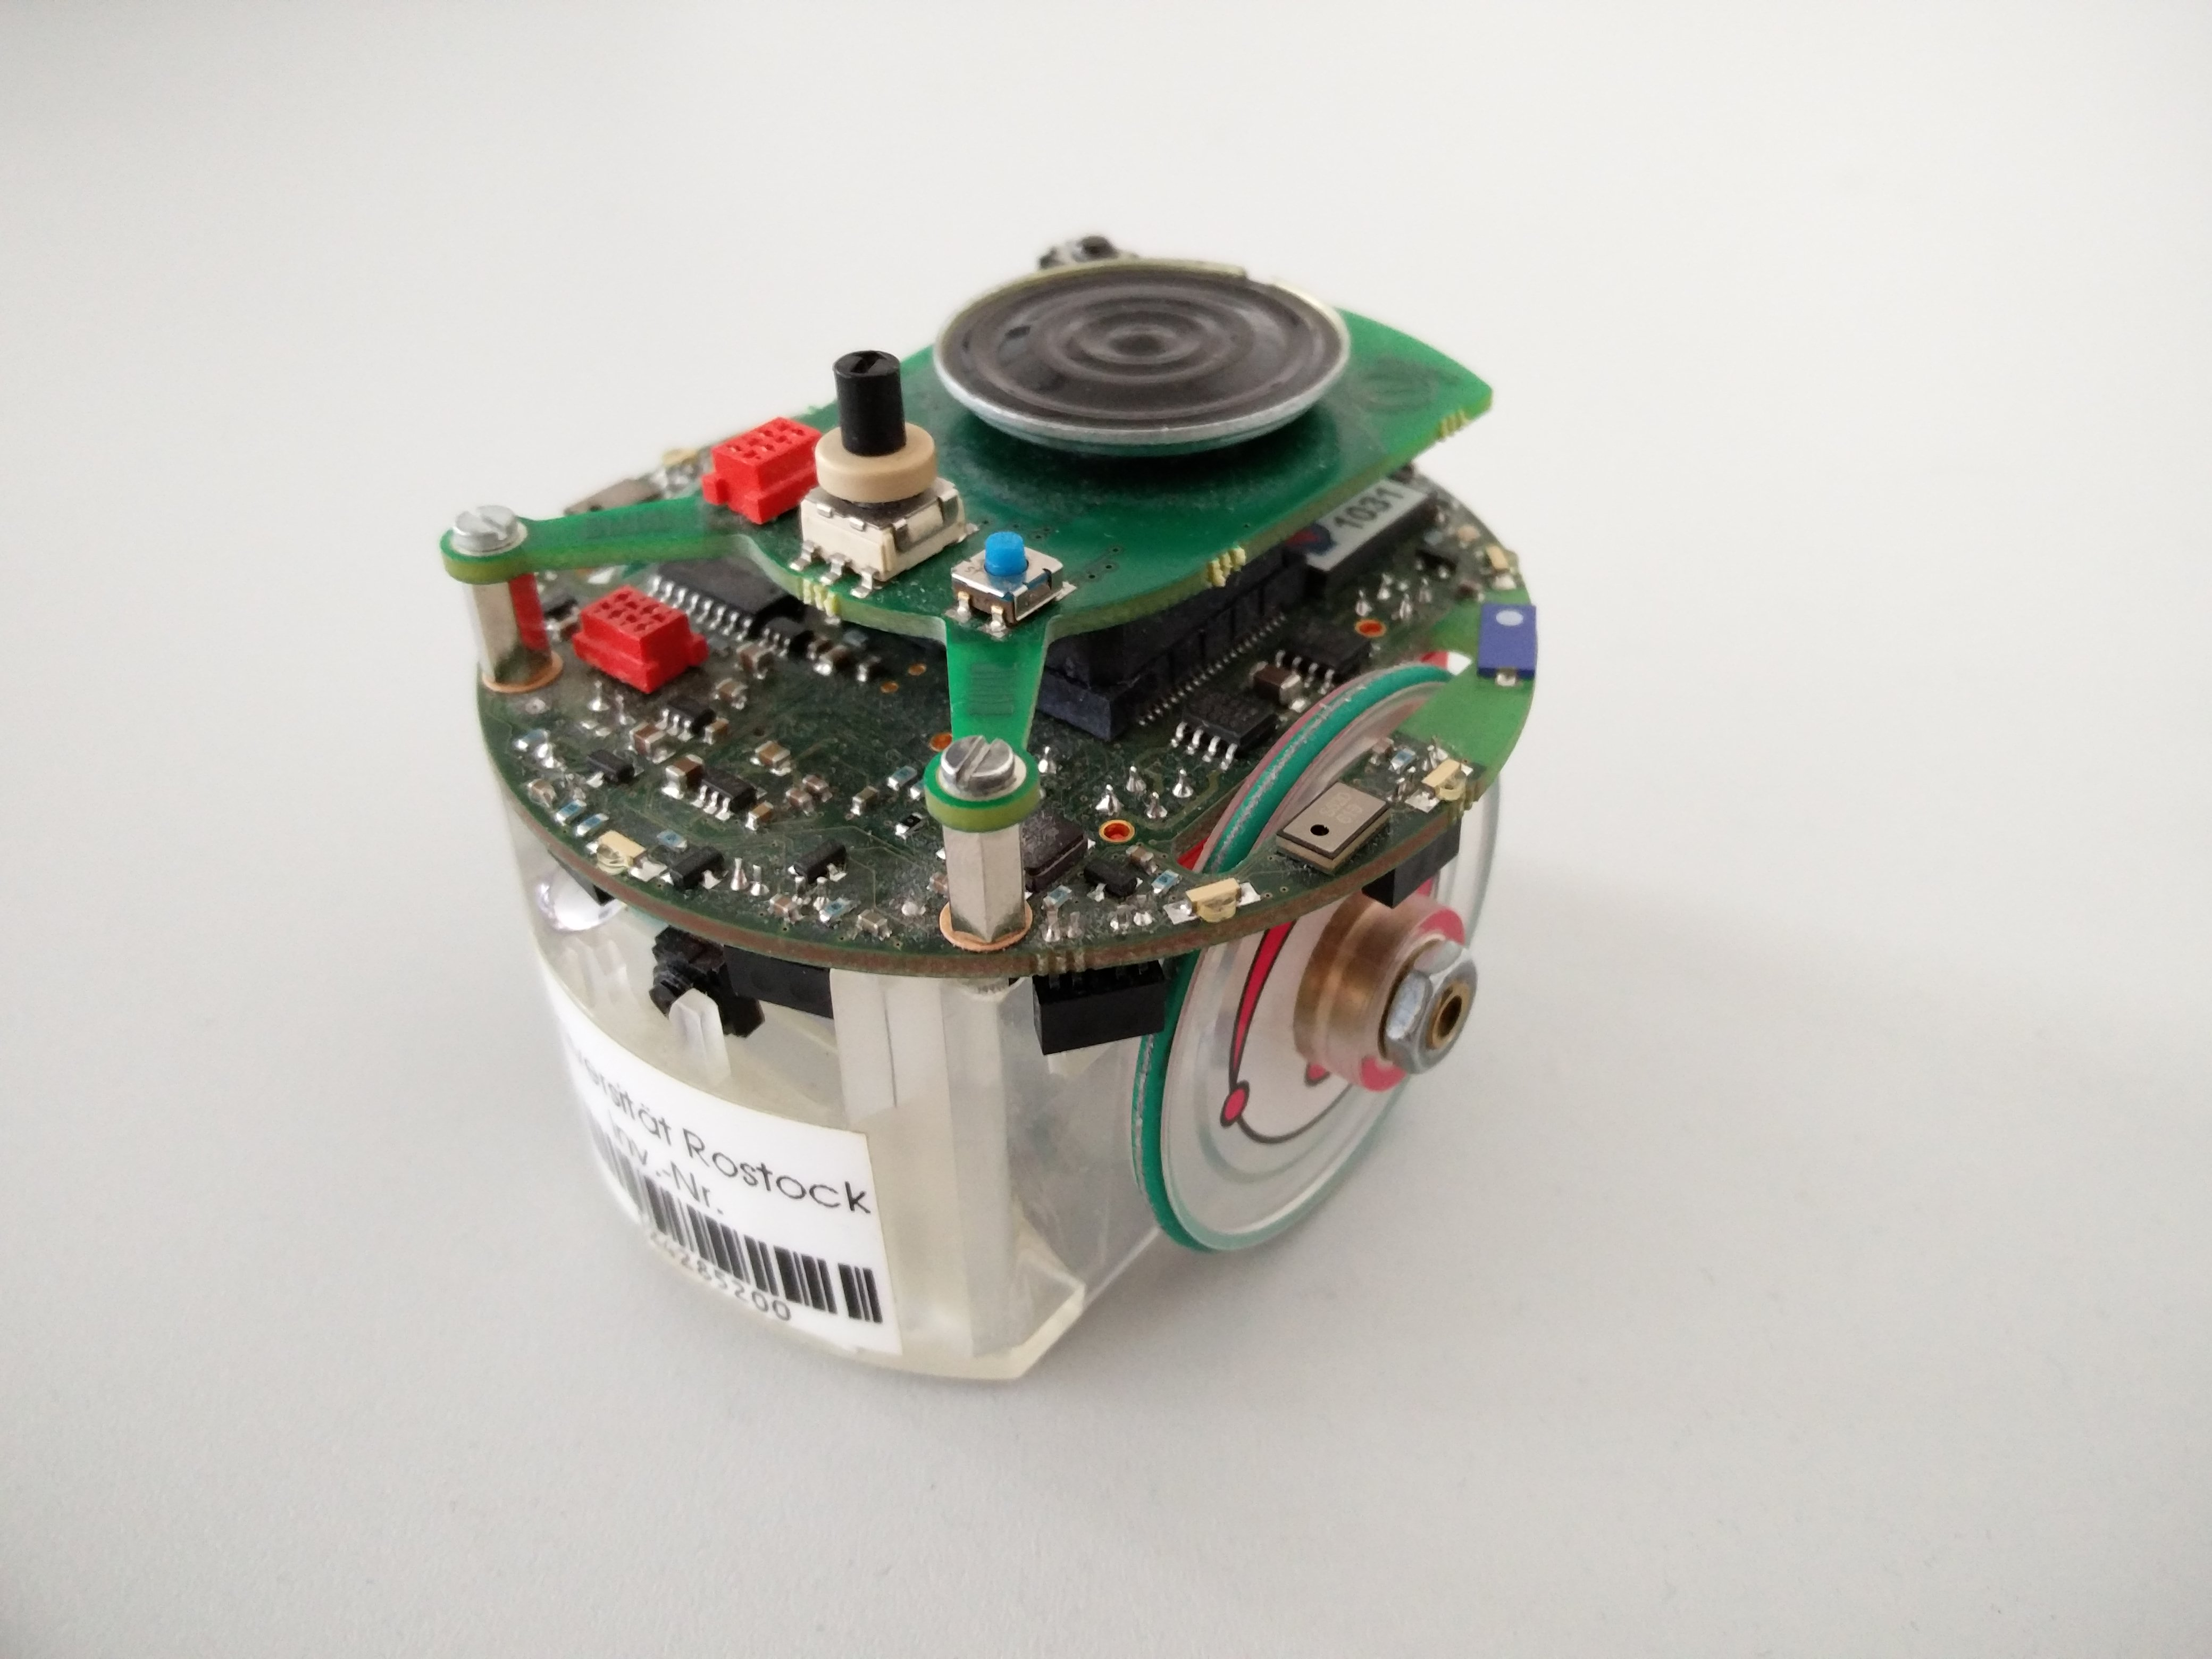
\includegraphics[width=\linewidth]{epuck.jpg}
	\caption{Photo of the E-Puck robot (front left view).}
	\label{fig:epuck_photo}
\end{figure}

In the following considerations, the sensor values are normalized to the range of $[0,1]\ni I$, a value of $1$ meaning that an obstacle is in close vicinity to the sensor, and $0$ that no backscattered IR signal is received at all. The motors' control signals are in the range of $[-1000,1000]\ni v$, with the extreme values meaning full speed backward and forward, respectively.

\begin{figure}[hbt]
	\centering
	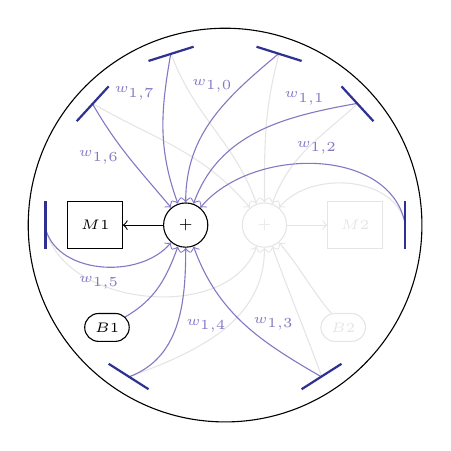
\begin{tikzpicture} 
	\tikzstyle{every node}=[font=\tiny]
	% basic structure
	\draw (0,0) circle [radius=2.5];
	\draw (1.3,-0.3)[irrelevantcolor] rectangle (2,0.3);
	\node ()[irrelevantcolor] at (1.65,0) {$M2$};
	\draw (-1.3,-0.3) rectangle (-2,0.3);
	\node () at (-1.65,0) {$M1$};
	% Adders
	\node (plus1) [draw, shape=circle] at (-0.5,0) {+};
	\draw [->] (plus1) to[out=180, in=0] (-1.3,0);
	\node (plus2) [draw, shape=circle, irrelevantcolor] at (0.5,0) {+};
	\draw [->,irrelevantcolor] (plus2) to[out=0, in=180] (1.3,0);
	% Arrows to second adder
	\draw [->,irrelevantcolor](0:2.29) to[out=100,in=50] (plus2);
	\draw [->,irrelevantcolor](42.5:2.29) to[out=222.5,in=70] (plus2);
	\draw [->,irrelevantcolor](72.5:2.29) to[out=255,in=90] (plus2);
	\draw [->,irrelevantcolor](107.5:2.29) to[out=290,in=110] (plus2);
	\draw [->,irrelevantcolor](137.5:2.29) to[out=330,in=130] (plus2);
	\draw [->,irrelevantcolor](180:2.29) to[out=280,in=250] (plus2);
	\draw [->,irrelevantcolor](237.5:2.29) to[out=20,in=270] (plus2);
	\draw [->,irrelevantcolor](302.5:2.29) to[out=110,in=290] (plus2);
	% Arrows to first adder
	\draw [->,weightcolor](72.5:2.29) to[out=220,in=90] node [near start, left, rotate=0] {$w_{1,0}$} (plus1);
	\draw [->,weightcolor](42.5:2.29) to[out=190,in=70] node [near start, above, rotate=0] {$w_{1,1}$} (plus1);
	\draw [->,weightcolor](0:2.29) to[out=100,in=50] node [midway, above, rotate=0] {$w_{1,2}$} (plus1);
	\draw [->,weightcolor](302.5:2.29) to[out=150,in=290] node [right, rotate=0] {$w_{1,3}$} (plus1);
	\draw [->,weightcolor](237.5:2.29) to[out=20,in=270] node [right, rotate=0] {$w_{1,4}$} (plus1);
	\draw [->,weightcolor](180:2.29) to[out=280,in=230] node [below, rotate=0] {$w_{1,5}$} (plus1);
	\draw [->,weightcolor](137.5:2.29) to[out=300,in=130] node [left, rotate=0] {$w_{1,6}$} (plus1);
	\draw [->,weightcolor](107.5:2.29) to[out=260,in=110] node [near start, left, rotate=0] {$w_{1,7}$} (plus1);
	% Sensors
	\draw [thick, sensorcolor](-7.5:2.3) -- (7.5:2.3);
	\draw [thick, sensorcolor](35:2.3) -- (50:2.3);
	\draw [thick, sensorcolor](65:2.3) -- (80:2.3);
	\draw [thick, sensorcolor](100:2.3) -- (115:2.3);
	\draw [thick, sensorcolor](130:2.3) -- (145:2.3);
	\draw [thick, sensorcolor](172.5:2.3) -- (187.5:2.3);
	\draw [thick, sensorcolor](230:2.3) -- (245:2.3);
	\draw [thick, sensorcolor](295:2.3) -- (310:2.3);
	% Biases
	\node (bias1)[draw,shape=rounded rectangle] at (-1.5,-1.3) {$B1$};
	\draw [->, weightcolor] (bias1) to[out=30, in=250] (plus1);
	\node (bias2)[irrelevantcolor,draw,shape=rounded rectangle] at (1.5,-1.3) {$B2$};
	\draw [->, irrelevantcolor] (bias2) to[out=130, in=310] (plus2);
\end{tikzpicture}
	\caption{Sketch of the E-Puck robot, with motors, sensors and weights of the left side.}
	\label{fig:epuck}
\end{figure}

In this scenario, the E-Puck shall provide an obstacle avoidance behaviour. Consider the following example as an explanation for the desired functionality: if one of the front right sensors register an approaching obstacle and therefore generate a value, motor $M_\mathrm{R}$ should speed up, while $M_\mathrm{L}$ should reduce its speed, which results in a left turn, away from the obstacle.

\section{Evolutionary Approach}

To find (near) optimal values for the weights $w$ with respect to a certain desired behaviour, evolutionary algorithms (EA) can be utilized.

The EA finds an extremal value of a fitness function $f$ over the search space by creating a population of individuals, containing parents and offspring. Each individual holds a genome equal to its position in the search space. In each evolution step, the parent individuals are copied or \emph{recombined}. The offspring is then randomly\footnote{by a Gaussian $\mathcal{N}(0,\sigma)$ distributed number} \emph{mutated}. The parents for the next generation are selected from the population according to the aforementioned fitness function. The EA strategy can be modified by changing the population size, selection method, mutation and recombination parameters.

In this scenario, a symmetric BV shall show a collision avoidance behaviour while driving around a maze. Referring to Eq.~(\ref{eq:motorequation}), the weights are chosen from the interval $[-1000,1000]\ni w$ accordingly. The search space is formed by the nine weights, thus limited to $[-1000,1000]^9$. The fitness function \mbox{$f:[-1000,1000]^9\to \mathbb{R}$} indicates, how well the BV moves around its environment. Thus, $f$ has to be evaluated over a certain time $T$:
\begin{equation}
	f = \sum\limits_T \tilde{f}.
\end{equation}
While in theory an integration, the total fitness is computed by a sum of multiple fitness contributions over a finite number of time steps. 

The fitness value $\tilde{f}$ of each individual time step should reward straight forward movement, and penalize both close distance to walls and irregular movement. Forward movement corresponds to a high \emph{average} speed between the two motors. In contrast, a high speed \emph{difference} indicates irregular movement and frequent turning. Nevertheless, turning is essential for avoiding obstacles, therefore this penalty is attenuated by the $\exp()$ function. The \emph{maximum} value of the proximity sensor readouts is utilized as an additional penalty. These components are connected via multiplication, so that the different physical units and orders of magnitude of the three terms can be omitted. This leads to the following fitness contribution of one time step:
\begin{equation}
	\tilde{f} = \left( v_\mathrm{L} + v_\mathrm{R} \right) \cdot \exp\left( - k_{\Delta v}|v_\mathrm{L}-v_\mathrm{R}| \right) \cdot \left(1- k_{I} \max\limits_i I_i\right)
	\label{eq:fitness_timestep} 
\end{equation}
The constants $k_{\Delta v}$, $k_I$ prevent the occurrence of negative values for the penalty factors of~(\ref{eq:fitness_timestep}). They also allow for a fine adjustment by weighting the different influences against each other.

In practice, to get an (mostly) unbiased fitness evaluation for each individual, for each time step the E-Puck should be placed at the same starting position in the maze manually. The fitness is then evaluated by driving around for a reasonably long time $T$. 

Here, $T\approx\SI{30}{\sec}$ was chosen. For the EA, the $(1+1)$ strategy was tested. A reasonable behaviour was reached after roughly fifty generations.


\section{Adaptive Learning}

Due to the random mutation, the EA is a undirected, and therefore a relatively slow strategy for optimizing an E-Puck Braitenberg Vehicle. The individual makes no learning progress whatsoever, and is eventually killed off by the selection algorithm. Additionally, the learning process heavily depends on the quality of the fitness function, which itself is depending on the current environment. The EA thus has a hard time reacting on changing environments, e.g. placing the robot in a maze with walls of different reflectivity.


To achieve a both adaptive and individual learning process, a combination of controller and value system was implemented, as shown in Fig.~(\ref{fig:adaptivelearningsketch}). The controller provides the basic behaviour by activating the motors according to Eq.~(\ref{eq:motorequation}) and the current weights.

\begin{figure*}[tbp]
	\centering
	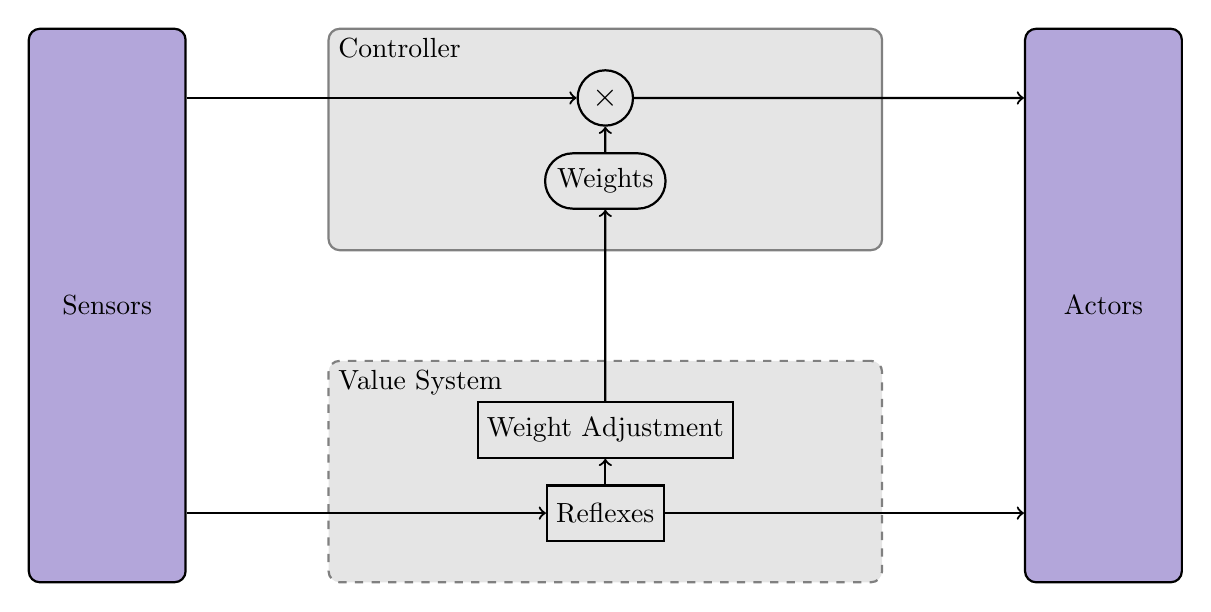
\begin{tikzpicture}
	\node (sensorblock) [outerblock] {Sensors};
	\path (sensorblock) + (18em,6em) node (controller) [midblocks] {};
	\path (controller) + (-10em,4em) node [below right] {Controller};
	\path (sensorblock) + (18em,-6em) node (valuesystem) [midblocks, dashed] {};
	\path (valuesystem) + (-10em,4em) node [below right] {Value System};
	\path (sensorblock) + (36em,0) node (Actors) [outerblock] {Actors};
	\path (valuesystem) + (0,-1.5em) node (Reflexes) [vsinnerblock] {Reflexes};
	\path (valuesystem) + (0,1.5em) node (Adjustment) [vsinnerblock] {Weight Adjustment};
	\path (controller) + (0,-1.5em) node (Weights) [cinnerblock] {Weights};
	\path (controller) + (0,1.5em) node (multiply) [cinnerblock] {\large $\times$};
	\draw [->,thick] (Reflexes) to (Adjustment);
	\draw [->,thick] (Adjustment) to (Weights);
	\draw [->,thick] (sensorblock.east |- multiply) -- (multiply);
	\draw [->, thick] (sensorblock.east |- Reflexes) -- (Reflexes);
	\draw [->, thick] (Reflexes) -- (Actors.west |- Reflexes);
	\draw [->, thick] (multiply) -- (Actors.west |- multiply);
	\draw [->, thick] (Weights) -- (multiply);
\end{tikzpicture}

	\caption{Block diagram of the implemented adaptive learning concept.}
	\label{fig:adaptivelearningsketch}
\end{figure*}

The value system's task is to simulate reward and punishment for a certain behaviour by adjusting the weights, as well as to provide reflexes for specific situations.

In this example, the value systems reacts to a collision with an obstacle. Usually, a collision $C$ is detected when any of the sensor values exceeds a certain threshold $\Theta_I$:
\begin{equation}
	C = \bigvee\limits_{i=0}^{N-1} I_i > \Theta_I. 
\end{equation}
During the testing of the adaptive algorithm, the E-Puck eventually got stuck at a convex corner in a way, that both sensors nearest to said corner did not reach $\Theta$. Therefore, a collision is also assumed, if both the squared norm of all sensor readouts is above a certain value $\Theta_A$, and the readouts of each individual sensor do not have a change bigger than a certain value $\Theta_B$ over a defined time.
\begin{equation}
	C = \sum\limits_{i=0}^{N-1} I_i^2 > \Theta_A \;\wedge\; \sum\limits_{i=0}^{N-1} (\Delta I_i)^2 < \Theta_B.
\end{equation}
However, this situation occurs very rarely. 
Both collision types are countered with a back-off reflex, meaning the robot moves away from the obstacle for a short time period.

For the first collision type, the weight of the sensor $I_m$ with the highest value is increased or decreased by a certain value $\Delta w$, depending on which side of the E-Puck the sensor is on, as the right motor's weights are the left motor's weights in reverse order:
\begin{align}
	w_m &\leftarrow w_m \pm \Delta w\label{eq:weightcorrection}
\end{align}

To prevent the weights from reaching too high magnitudes, they are normalized after the correction~(\ref{eq:weightcorrection}), if necessary. If the squared norm of the sensor weights is larger than a value $\Theta_W$, i.e.
\begin{equation}
	W = \sum\limits_{i=0}^{N-1} w_i^2 > \Theta_W,
\end{equation}
the weights are normalized accordingly:
\begin{equation}
	w_i \leftarrow w_i \cdot \frac{\Theta_W}{W}.
\end{equation}
Here, a maximum norm of $\Theta_W=3\cdot 10^6$ limits each weight to roughly $1000$. A value of $\Delta w = 150$ was found suitable for the correction value. The bias is kept constant at $w_\text{bias} = 150$.

The frequency of the value system's interventions decreases over time, as the controller adapts better and better. In this scenario, a reasonable controller adaptation was reached after roughly thirty interventions or four minutes. After that, the value system only activates sporadically, to free the E-Puck BV from delicate situations. The adaptive learning therefore is by orders faster than the evolutionary approach.


\end{document}
	